%<code>

\documentclass[11pt,Times]{article}
%\usepackage[sort&compress,numbers]{natbib}
\usepackage{float,natbib}

\usepackage{amsmath, amsfonts, amsthm}
\usepackage{enumerate}
\usepackage{geometry} % see geometry.pdf on how to lay out the page. There's lots.
%\geometry{a4paper} % or letter or a5paper or ... etc
% \geometry{landscape} % rotated page geometry
\usepackage{graphicx,subfigure}
\usepackage{color}
\usepackage{hyperref}
\usepackage{setspace}

\usepackage{bm}

\usepackage{geometry}
\geometry{top=1in, bottom=1.5in, left=1.in, right=1.in}

\def\cite{\citep}
\def\citeN{\citet}  %in-text
\def\citeNP{\citep} % parances.

%\definecolor{gray}{RGB}{175,175,175}
\def\tcr{\textcolor{red}}
\def\tcb{\textcolor{blue}}
\def\ii{{(i)}}
\def\kk{{(k)}}
\def\Theta{\xi}
%\def\dir{/Users/yguan/work/2layer/latex}
\def\dir{.}

%\onehalfspacing
\begin{document}

%%%%%%%%%%%%%%%%%%%%%%%%%%%%%%



%% For titles, only capitalize the first letter

\title{Infer realized kinship via latent identity-by-descent states}

\author{Yongtao Guan and Daniel Levy \protect\\  National Heart, Lung, and Blood Institute}
\date{}
%% The \maketitle command is necessary to build the title page.
\maketitle

%%%%%%%%%%%%%%%%%%%%%%%%%%%%%%%%%%%%%%%%%%%%%%%%%%%%%%%%%%%%%%%%


%% When adding keywords, separate each term with a straight line: |
%\keywords{linkage disequilibrium | local ancestry | haplotype-phenotype | association}

\def\e{{\mathbf{\epsilon}}}
\def\u{{\mathbf{u}}}
\def\x{{\mathbf{x}}}
\def\X{{\mathbf{X}}}
\def\g{{\mathbf{g}}}
\def\al{{\mathbf{\alpha}}}
\def\ga{{\mathbf{\gamma}}}
\def\y{{\mathbf{y}}}
\def\bb{{\mathbf{\beta}}}
\def\a{{\mathbf{a}}}
\def\z{{\mathbf{z}}}
\def\Z{{\mathbf{Z}}}
\def\W{{\mathbf{W}}}
\def\Q{{\mathbf{Q}}}
\def\U{{\mathbf{U}}}
\def\D{{\mathbf{D}}}
\def\K{{\mathbf{K}}}
\def\S{{\mathbf{S}}}

%\newpage
\begin{abstract}
All humans are related to one another through the shared common ancesters, thus all people are inbred to various degrees. Therefore it is prudent to account for inbreeding when inferring kinship between individuals. We present a method Kindred that model joint genotype distributions through latent IBD states, which fully describes all possible allele sharing between two individuals. By inferring the probabilities of the latent states Kindred can infer kinship and inbreeding coefficients with high accuracy and efficiency. The latent IBD states model can show that genotype correlation between two individuals is expected to be twice their kinship. Kindred can estimate kinship on a genomic region that have enough SNPs to estimate joint genotype proportions. By choosing a set of SNPs that have the same distribution in allele frequencies across diverse populations, Kindred can infer kinship between recently admixed individuals.   
\end{abstract}

\newpage
\section{Introduction}
Kinship (denoted by $\phi$) is the probability that two alleles sampled each from two individuals are identical by descent (IBD).  Kinship between two individuals is the inbreeding coefficient (denoted by $F$) of their (hypothetical) children. In addition, between one and oneself (or between monozygotic twins) $\phi = (1+F)/2$~\cite{wright.22}.  Therefore, we treat inbreeding as a derived concept (and quantity) and will not discuss it separately here. Kinship estimated from genotype data is called realized kinship. Due to stochastic nature of recombination and gamete segregation, realized kinship may have significant variation from pedigree estimates~\cite{visscher.etal.06}.  Estimating realized kinship is an important problem in human genetics (e.g., in disease mapping) and animal and plant genetics (e.g., in breeding design). 
%

In an effort to study gene IBD, \citet{jacquard.72} documented $9$ IBD states between any two individuals on a pedigree. These IBD states are partially observable on a pedigree, and the mean probabilities of each state can be computed purely based on a pedigree.  These IBD states are completely latent between two individuals not linked on a known pedigree.  \citet{thompson.13} made connection between the Jacquard IBD states and the Ewen's sampling partition formula in coalescence, and provided the joint distribution of genotypes between two individuals conditioning on latent gene IBD states. These formed basis for our work here to infer latent IBD states between two individuals via joint genotype distribution and hence their kinship.   


Existing methods on kinship estimation, such as King~\cite{king} and that implemented in pLink~\cite{plink}, ignore the possible inbreeding of each sample. Inbreeding can affects the amount homozygous markers in the genome, and hence the length of homozygous run; not modeling inbreeding coefficients evidently bias kinship estimates. 
%For example, two unrelated but slightly inbred genomes will have nonzero kinship estimates. 
The classical method to estimate kinship is through genetic relatedness matrix (GRM) or genotype correlation between two samples~\cite{eigenstrat, gcta, wang.etal.17}. Although the diagonal entries of GRM is well justified with expectation $1+F$ (twice the kinship between one and oneself), the off-diagonal terms, which suppose to be twice the kinship, their theoretical justification is difficult to pin down. We provide justification in this paper through latent IBD states. 

We present Kindred that estimate kinship through inferring the probabilities of latent $9$ Jacquard IBD states.  Because of linear dependence, only four IBD states whose probabilities can be uniquely determined, the other five IBD states their probabilities are linearly dependent. But interestingly, certain linear combinations of those probabilities are invariant, which happen to guarantee a unique kinship estimate.  Kindred can be applied to sliding windows of SNPs to infer local kinship, and by curating a set of SNPs that have the similar allele frequency distribution in diverse populations, Kindred can be applied to admixed individuals.  


%Kinship inferred from genetic data is called realized kinship, in comparison to a kinship obtained from a pedigree relationship, which is the expected kinship. Due to stochastic nature of recombination and gamete segregation, realized kinship can have significant variation. For example, although the mean kinship coefficient first cousins is $0.0625$, the standard deviation is $0.0243.$ Realized kinship can also vary across chromosomes. 

%Kinship is a concept based on gene identical by descent (IBD), while IBD implicitly refer to an ideal population that is homogeous and outbred.  
%An direct relevance is the allele frequencies of the ideal reference population, as allele frequencies affect how likely SNPs are homozygous, affect centering and normalization SNPs in GRM calculation.  
%A curated set of allele frequencies is a good community effort.  we used 1000 Genomes dataset and selected SNPs that have similar allele frequencies between continental populations (small Fst values).This makes our method applicable to majority of populations, particularly recently admixed populations, at cost of increased uncertainty for descents of continental populations due to smaller numbers of SNPs.  Since we only used counts data, the computation is highly efficient compared to other haplotype based method. 

%In this study, we show that, as the consequence of Beyas rule, we can infer the (realized) probabilities of the latent Jacquard IBD states based on the joint genotypes, and consequently obtain the kinship estimates between two individuals and their respective inbreeding coefficients.  This latent states model can be used to confirm the validity of the popular genetic relatedness matrix (GRM), which is widely used in linear mixed model and heritability estimation, is indeed a function of kinship and inbreeding coefficients. 

%For individual j, the inbreeding coefficient $F_ j$ is the probability that its two alleles at a given locus are ibd. The kinship, or coancestry, coefficient $\phi_{ij}$ for individuals i and j is defined here as the average of the four ibd probabilities for one allele from each individual. It follows that the kinship of individual j with itself is $(1 + F_ j)/2$. (cite Goudet et al.)
%The kinship between parents is the inbreeding coefficient of the their children~\cite{thompson 2013 genetics}. 


\newpage
\section{Results}

\subsection{Latent IBD states model}
At an arbitrary marker, there are $15$ detailed IBD states between four alleles of two individuals.   
If the parental origin of an allele is not an interest, these $15$ states can be reduced to $9$ condensed IBD states~\cite{jacquard.72,thompson.13}. 
Here we work with the $9$ condensed identity states. Conditional on each state, we distribution of joint genotypes for a bi-allelic SNP is given in Table~\ref{distr}. Note this distribution is a bi-allelic special case of what's presented four allelic case in~\cite{thompson.13}. 

\begin{figure}[htbp]
\begin{center}
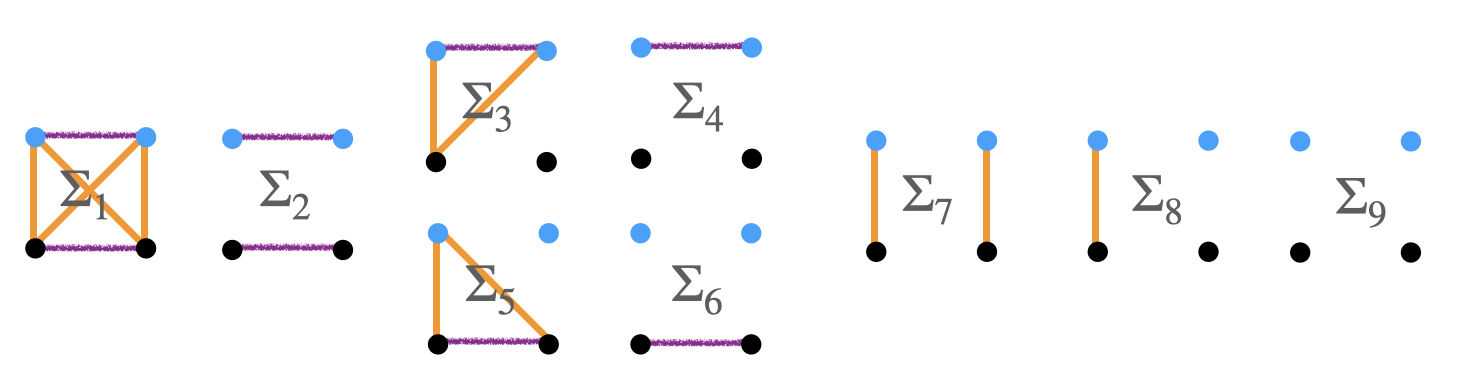
\includegraphics[width=0.8\textwidth]{jacquard.png}
\caption{Nine possible IBD sharing between two individuals. Two alleles of individual $1$ were labelled as blue and two alleles of individual $2$ were in black.  Two alleles IBD within an individual were connected via a purple segment. Two alleles IBD between individuals were connected by an orange segment. $\Sigma_7, \Sigma_8,$ and $\Sigma_9$ are two non-inbreed individuals share two, one, and zero alleles IBD respectively.  These are colored re-rendering of Table 2 in~\cite{jacquard.72}.}
\label{j9}
\end{center}
\end{figure}

\begin{table}[htp] 
\begin{center}
\begin{tabular}{lllllllll|ll}
 $\Sigma_1$ &  $\Sigma_2$ &  $\Sigma_3$ &  $\Sigma_4$ &  $\Sigma_5$ &  $\Sigma_6$ &  $\Sigma_7$ &  $\Sigma_8$ &  $\Sigma_9$ &G1 & G2 \\
\hline 
 $p$ & $p^2$ & $p^2$ & $p^3$ & $p^2$ & $p^3$ & $p^2$ & $p^3$ & $p^4$ & AA &AA \\       
 $0$ & $0$ & $pq$ & $2p^2q$ & $0$ & $0$ & $0$ & $p^2q$ &$2p^3q$ &AA &AB  \\
 $0$ & $pq$ & $0$ & $pq^2$ & $0$ & $p^2q$ & $0$ & $0$ &$p^2q^2$ &AA &BB \\
 $0$ & $0$ & $0$ & $0$ & $pq$ & $2p^2q$ & $0$ & $p^2q$ &$2p^3q$ & AB &AA   \\
$0$ & $0$ & $0$ & $0$ & $0$ & $0$ & $2pq$ & $pq$ &$4p^2q^2$ & AB &AB   \\
 $0$ & $0$ & $0$ & $0$ & $pq$ & $2pq^2$ & $0$ & $pq^2$ &$2pq^3$ & AB &BB \\
$0$ & $pq$ & $0$ & $p^2q$ & $0$ & $pq^2$ & $0$ & $0$ &$p^2q^2$ & BB &AA   \\
 $0$ & $0$ & $pq$ & $2pq^2$ & $0$ & $0$ & $0$ & $pq^2$ &$2pq^3$ &BB &AB   \\
 $q$ & $q^2$ & $q^2$ & $q^3$ & $q^2$ & $q^3$ & $q^2$ & $q^3$ & $q^4$ &BB &BB \\       
%\hline 
%& && 0 & 4 & 1 & 3 & 1 & 3 & 0 & 1 & 2 \\
  \end{tabular}
  \caption{Joint genotype distribution for each latent IBD states, reproduced from Table 3 of~\cite{thompson.13}. Each of the nine columns labelled by $\Sigma_j$ corresponds to a latent state in Figure~\ref{j9}. The joint genotypes are listed in columns G1 and G2 where the order matters. $p$ denotes the frequency of A allele and $q$ frequency of B allele, and $p+q=1$. Note each column labelled by $\Sigma_j$ sums to $1$. When G1 and G2 are the genotypes of the same individual, only $\Sigma_1$ and $\Sigma_7$ are relevant. When inbreeding is ignored, only last three $\Sigma$ columns are relevant.}
  \label{distr}
  \end{center}
\end{table}


\begin{table}[htp] 
\begin{center}
\begin{tabular}{lll|lllllll}
G1 & G2 & H & $\Sigma_1$ &  $\Sigma_2$ &  $\Sigma_{3,5}$ &  $\Sigma_{4,6}$  &  $\Sigma_7$ &  $\Sigma_8$ &  $\Sigma_9$ \\
\hline 
AA &AA &0 & $p$ & $p^2$ & $p^2$ & $p^3$  & $p^2$ & $p^3$ & $p^4$ \\       
AA &BB &4 & $0$ & $2pq$ & $0$ & $pq$   & $0$ & $0$ &$2p^2q^2$ \\
BB &BB  &0& $q$ & $q^2$ & $q^2$ & $q^3$  & $q^2$ & $q^3$ & $q^4$ \\       
AB &AA &2 & $0$ & $0$ & $pq$ & $2p^2q$  & $0$ & $2p^2q$ &$4p^3q$ \\
AB &AB &0 & $0$ & $0$ & $0$ & $0$  & $2pq$ & $pq$ &$4p^2q^2$ \\
AB &BB &2& $0$ & $0$ & $pq$ & $2pq^2$  & $0$ & $2pq^2$ &$4pq^3$ \\
\hline 
& && 0 & 4 & 2 & 6 & 0 & 1 & 2 \\
  \end{tabular}
  \caption{}\label{distr}
  \end{center}
\end{table}


%We first show that GRM calculation for kinship is consistent with the latent IBD model (we call it latent IBD model).
Kinship can be computed from latent IBD probabilities as follows~\cite{jacquard.72}. 
\begin{equation}\label{e1}
\begin{aligned}
\phi &= \Delta_1 + \frac{1}{2}(\Delta_3+\Delta_5+\Delta_7) + \frac{1}{4} \Delta_8  \\
%F_1 &= \Delta_1 + \Delta_2 + \Delta_3 + \Delta_4 \\
%F_2 &= \Delta_1 + \Delta_2 + \Delta_5 + \Delta_6 \\
\end{aligned}
\end{equation}
The fractions in Equation~\eqref{e1} comes from one (paternal and maternal) equivalence IBD states to $\Sigma_3, \Sigma_5,$ and $\Sigma_7$ folded into them, and three equivalent IBD states to $\Sigma_8$ folded into it. (That is how $15$ states were reduced to $9$.)  Inbreeding coefficients can also be computed from latent IBD probabilities~\cite{jacquard.72}. 
\begin{equation}\label{e2}
\begin{aligned}
%\phi &= \Delta_1 + \frac{1}{2}(\Delta_3+\Delta_5+\Delta_7) + \frac{1}{4} \Delta_8  \\
F_1 &= \Delta_1 + \Delta_2 + \Delta_3 + \Delta_4 \\
F_2 &= \Delta_1 + \Delta_2 + \Delta_5 + \Delta_6 \\
\end{aligned}
\end{equation}


Let $X$ and $Y$ denote allele counts of genotypes $G1$ and $G2$ in Table~\ref{distr}, $p$ is allele frequency of $A$ allele and $q=1-p$, and consider 
\begin{equation}\label{grm}
\begin{aligned}
\frac{(X-Y)^2}{2pq} = \frac{(X-2p)^2}{2pq} + \frac{(Y-2p)^2}{2pq} - 2 \frac{(X-2p) (Y-2p)}{2pq}.
\end{aligned}
\end{equation}
Note $Q = \frac{(X-2p) (Y-2p)}{2pq}$ is the quantity calculated in GRM. The left hand side in Equation~\eqref{grm} can be directly computed in light of Table~\ref{distr}, and we get $LHS=4\Delta_2 + \Delta_3 + 3\Delta_4 + \Delta_5 + 3\Delta_6 + \Delta_8 + 2\Delta_9$. Identifying the right hand side is $1+F_1 + 1+ F_2 -  2Q$ and plugging $F_1$ and $F_2$ in Equations~\eqref{e2} to get $RHS = 2 + 2\Delta_1 + 2\Delta_2 + \Delta_3+\Delta_4+\Delta_5+\Delta_6 - 2Q$. Equating $LHS = RHS$ and making use the identity $\sum_{j=1}^9\Delta_i = 1$, to get $Q = 2 \Delta_1 + (\Delta_3+\Delta_5+\Delta_7) + \frac{1}{2} \Delta_8 = 2\phi$, as defined in Equation~\eqref{e1}.   Corollarily, since $Q = (1+F_1 + 1 + F_2 - LHS)/ 2$, not accounting for inbreeding effectively setting $F_1=F_2=0$, which will reduce $Q$ and causing negative entries in GRM.  
  


%Suppose all bi-allelic SNPs have the same allele frequency, and counts for each genotype combinations are $n_{1}, n_{2}, \dots, n_{9}$, then we can write the log likelihood 
%$$ l (\Delta_1, \dots, \Delta_9) \propto {n_{1}} \log \theta_{1} +\dots + {n_{9}} \log \theta_{9} $$ 

%Goudet J, Kay T, Weir BS. How to estimate kinship. Mol Ecol. 2018 Oct;27(20):4121-4135. doi: 10.1111/mec.14833. Epub 2018 Sep 7. PMID: 30107060; PMCID: PMC6220858.

\vspace{.2in} 
With Table~\ref{distr}, we can model the observed genotypes as emitted from the mixture of latent states and to infer the mixture proporotion $\Delta$ and obtain an kinship estimate from Equation~\eqref{e1}. We start by considering a subset of SNPs with allele frequency $p$ so that they share the same matrix $\Sigma_p$ connecting joint genotype counts and the mixture probabilities of latent states. 
%\begin{equation}
\begin{align}
(n_{p,1}, \dots, n_{p,9}) &\sim \mbox{Multinomial}(\theta_{p,1}, \dots, \theta_{p,9}) \label{mn}\\
\S_p \Delta  &= \hat\theta_p \label{lse}
\end{align}
%\end{equation}
where $\S_p = (\Sigma_1, \dots, \Sigma_9)$ (Table~\ref{distr}), $n_{p,1}$ is count of $AA\;AA$ genotypes of allele frequency $p$ and $n_{p,9}$ is count of $BB\;BB$ of allele frequency $p$ (Table~\ref{distr}). The maximum likelihood estimate for $\theta_{p,1}, \dots,  \theta_{p,9}$ are $\hat{\theta}_{p,1}=n_1/\sum{n_{p,j}}, \dots, \hat{\theta}_{p,9} = n_{p,9}/\sum{n_{p,j}}$.  
%(With a Bayesian hat, we can specify Dirichlet prior on the multinomial model to obtain posterior estimates that are similar to MLE estimates. Since we have overwhelmingly large counts, Bayesian and MLE estimates are almost identical on reasonable choice of priors.)
We can solve a linear system $\S_p \Delta = \hat\theta_p$ with constraint $\Delta_j \ge 0$ and $\sum_{j=1}^9\Delta_i = 1$ to obtain least square estimates $\hat{\Delta}$ and obtain $\phi$ according to Equation~\eqref{e1}. 
%Note here we effectively treat $\hat\theta$ as observed and seeking a least square fit to estimate $\Delta$.  
We can of course attach another matrix $\S_{p'}$ to $\S_p$ and $\hat{\theta'}$ to $\hat{\theta}$ and use SNPs of allele frequency $p'$ to increase quality of $\hat{\Delta}$ estimates. 

\vspace{.1in} 
In fact, we can do so for each SNP. For the $i$th SNP with allele frequency $p_i$, we have $\S_{p_i}$ matrix and $\hat{\theta}=e_i$ where $e_i$ has a single entry equals $1$ (depending on the joint genotypes) and other $8$ entries equal $0$.  For each SNP, we append $9$ rows to the design matrix $\S$ and $9$ rows of a (trivial) genotype frequency vector to $\hat\theta$. For total $m$ SNPs, $\S$ is an $9m \times 9$ matrix, and $\hat{\theta}$ is an $9m$ vector, and we fit the model with the simplex constraint to obtain $\hat{\Delta}$.  
%
Now consider $\S^t \S \cdot \Delta = \S^t \hat\theta$, which shall have the same solution of $\S \Delta = \hat\theta$.  Let $\S^t \S = \sum_i^m \S_{p_i}^t \S_{p_i}$ and $\S^t \hat\theta = \sum_i^m \S_{p_i}^t e_i$. If all $p_i = p$, the system reduce to $\S_p^t \S_p \Delta =\S_p^t \hat\theta_{p}$ which have the same solution as Equation~\eqref{lse}.  We can efficiently compute $\sum_i^m \S_{p_i}^t S_{p_i}$, by binning $p_i$ to the second decimal place and do a weighted sum after counting the number of SNPs in each allele frequency bin.  Similarly  $\sum_i^m \S_{p_i}^t e_i$ can be efficiently computed. 
%For a preselected set of SNPs, we can compute integration $\int_{0}^1\S_{p}^t \S_p f(p) dp$, where $f(p)$ is the density and the integration is done entry-wise. 



\vspace{.1in} 
It can be verified that there are two linear dependence in $\S_p$. One is  $\Sigma_2 + 2 \Sigma_8 = \Sigma_4 + \Sigma_6 + \Sigma_7$ and the other is $pq (\Sigma_1+\Sigma_2- 2\Sigma_3 - 2\Sigma_5 + 2\Sigma_7)  =  \Sigma_7 - 2 \Sigma_8 +  \Sigma_9$. But since the second linear dependence is a function of allele frequency, it disappears when SNPs of different allele frequencies were used in calculation. Nevertheless, by virtual of the first dependence, the solution to the system $\S \Delta = \hat\theta$ is not unique. Let $\S^{+}$ be Moore-Penrose inverse of $\S$, then $\Delta = \S^{+} \hat\theta + (I - \S^{+} \S) v$ for any vector $v$~\cite{penrose.55}.  Denote $C = (I - \S^{+} \S) v$,  it can be verified that  

\begin{equation}\label{C}
\begin{aligned}
C_1 =C_3=C_5=C_9 &= 0 \\
C_2  &=  \frac{1}{8} v_2 -  \frac{1}{8} v_4 -  \frac{1}{8} v_6 -  \frac{1}{8} v_7 +  \frac{1}{4} v_8 \\  
C_4 =  C_6 = C_7 &=  - \frac{1}{8} v_2 +  \frac{1}{8} v_4 +  \frac{1}{8} v_6 +  \frac{1}{8} v_7 -  \frac{1}{4} v_8 \\
%C_6 &= - \frac{1}{8} v_2 +  \frac{1}{8} v_4 +  \frac{1}{8} v_6 +  \frac{1}{8} v_7 -  \frac{1}{4} v_8 \\
% C_7 &=   - \frac{1}{8} v_2 +  \frac{1}{8} v_4 +  \frac{1}{8} v_6 +  \frac{1}{8} v_7 -  \frac{1}{4} v_8 \\
  C_8 &= \frac{1}{4} v_2 - \frac{1}{4}  v_4 - \frac{1}{4}  v_6 - \frac{1}{4}  v_7 + \frac{1}{2}  v_8. \\
\end{aligned}
\end{equation}
We make the following observations based on Equation~\eqref{C}.  First,  $\Delta_1, \Delta_3, \Delta_5$, and $\Delta_9$ are not affected by $v$ and these components have unique solutions. Second, $C_2 + C_4 = 0$, $C_2+C_6 = 0$ and $C_7 + \frac{1}{2}C_8 = 0$, which means,  although $\Delta_2, \Delta_4, \Delta_6, \Delta_7,$ and $\Delta_8$ have infinite many solutions, $\Delta_2+\Delta_4 $, $\Delta_2+\Delta_6$, and  $\Delta_7 + \frac{1}{2}\Delta_8$ however are invariant. Third, as a consequence to the first two observations, $\phi$ in Equation~\eqref{e1} and $F_1$ and $F_2$ in Equation~\eqref{e2} are unique. 
 %Which means any solution to  $A \Delta = b$, among all possible solutions, produces correct estimates of kinship and inbreeding coefficients.  
% Fourth, when we seek a solution to $\S \Delta = \hat\theta$, we only need to enforce $\Delta_1, \Delta_3, \Delta_5$, and $\Delta_9$ to be nonnegative. This means least square fit might be sufficient, as oppose to the more costly nonnegative least square fit or bounded value least square fit.  
Finally, from the nonnegative constraints on $\Delta$'s, we have when $\Delta_2 = 0 \mbox{ and } \Delta_4 = 0$, or $\Delta_2 = 0 \mbox{ and } \Delta_6 = 0$, or  $\Delta_2 = 0 \mbox{ and } \Delta_7 = 0$, or $\Delta_7 = 1$, the solutions are unique.  

\newpage
\vspace{.2in} 
We used ped-sim~\cite{ped-sim} to simulate pedigrees with 1000 genomes genotypes as founders to obtain full siblings, parent offspring, half siblings, first-degree, second-degree, and third-degree cousins. 
demonstrate that it works for admixed samples, 

bcftools view cousin.chb-chs.vcf.gz --regions 6 | ./kindred -v - -o chr6  

\newpage
\section{Discussion}
Kinship inference is at the center of disease mapping in human genetics, it has been used for controlling for population stratification and (cryptic) relatedness in genome-wide association studies~\cite{eigenstrat, thornton.mcpeek.10,emmax, zhou.stephens.12, chen.etal.16}. 

The classic genomic relationship matrix (GRM) estimator  estimates kinship through the empirical correlation of genotypes. 
Since $\phi$ and $F$ are probabilities by definition, the diagonal entries in GRM estimates $\ge 1$ (expectation $1+F$) and off diagonal entries $\ge 0$ (defined as $2\phi$). 
But in practice we often observe diagonal entries $<1$ and off diagonal entires $<0$. 

A recent study shows that GRM based on genotype correlation have bias due to inaccurate allele frequency used in calculating correlations. 
Another need to call for curated allele frequencies is the kinship estimation for admixed samples. 
The kinship in the sample will bias the allele frequency estimates, methods have been developed to take into account of kinship when inferring allele frequencies. 


%This article focuses on pedigree-free estimation of realized kinship in a homogenous population.

%The PLINK (Purcell et al. 2007) method-of-moments estimator  estimates realized kinship from the k coefficients; the proportion of genome at which two noninbred individuals share 0, 1, or 2 IBD genes.


For admixed samples,  find a subset of SNPs that have the same (uniform) distribution in allele frequency in different populations. 
need to use curated allele frequency. as to estimate allele frequency without bias, one has to take into account of genetic relatedness in the sample when estimating allele frequencies. Of course, this problem can be alleviated by an iterative procedure where one conditioning relatedness to estimate allele frequency and use estimated allele frequency to re-estimate genetic relatedness, repeat until both estimates converge. 

%https://www.ncbi.nlm.nih.gov/pmc/articles/PMC2556426/
%As a consequence, grandchildren vary in the proportion of DNA they inherit from each of their four grandparents, and although the mean F coefficient of the offspring of first cousins is 0.0625, the standard deviation is 0.0243.


As a consequence, grandchildren vary in the proportion of DNA they inherit from each of their four grandparents, and although the mean F coefficient of the offspring of first cousins is 0.0625, the standard deviation is 0.0243.
Several studies in consanguineous or small, isolated populations with above average levels of parental relatedness have found evidence for a genome-wide effect of homozygosity on coronary heart disease,29–31 cancer,29,32–34 blood pressure,10–17 and LDL cholesterol.15

we can compute $L_2$ distance between two individuals from the kinsip. 
Finally, what if everyone is slightly inbred thus the volume the GRM is larger than $1$? will this inflate the heritability estimates in GCTA? 

\newpage
\section{Method}
\subsection{simulate genotypes of different relatedness using ped-sim}
We first combine CHB and CHS into one sample, computed pairwise kinship and removed samples such that pairwise kinship is $< 0.001$. 
We then simulate different relatedness using ped-sim with the recombination rate provided by ped-sim and 


%\begin{verbatim}
%ped-sim -d grandparents.def -m refined_mf.simmap -i 1000g.thin1000-2SNPs-chb-chs-chrall.recode.vcf.gz --pois -o grandparents --nogz
%ped-sim -d half-sibling.def -m refined_mf.simmap -i 1000g.thin1000-2SNPs-chb-chs-chrall.recode.vcf.gz --pois -o half-sibling --nogz
%ped-sim -d first-cousin.def -m refined_mf.simmap -i 1000g.thin1000-2SNPs-chb-chs-chrall.recode.vcf.gz --pois -o first-cousin --nogz
%ped-sim -d second-cousin.def -m refined_mf.simmap -i 1000g.thin1000-2SNPs-chb-chs-chrall.recode.vcf.gz --pois -o second-cousin --nogz
%ped-sim -d third-cousin.def -m refined_mf.simmap -i 1000g.thin1000-2SNPs-chb-chs-chrall.recode.vcf.gz --pois -o third-cousin --nogz
%\end{verbatim} 

\subsection{Bayes factor of linear mixed model}
Consider a linear model 
\begin{equation} \label{M1}
\begin{aligned}
M1: \y &= \W \alpha  + \e \\
\alpha &\sim MVN(0,  \tau^{-1}  V_W) \\
%\u &\sim MVN_m(0, \lambda \tau^{-1} K) \\
\e &\sim MVN_n(0, \tau^{-1} I_n)
\end{aligned}
\end{equation}
where $\W$ is a $n\times w$ representing $w$ nuisance covariates.    Adding a random effect $\u$ we have a new model 
%
\begin{equation} \label{M2Z}
\begin{aligned}
M2Z: \y &= \W \alpha  + \Z \u + \e \\
%\alpha &\sim MVN(0, \tau^{-1} V_0) \\
\u &\sim MVN_m(0, \tau^{-1} \lambda K) \\
%\e &\sim MVN_n(0, \tau^{-1} I_n)
\end{aligned}
\end{equation}
where $Z$ is $n \times m$ matrix presenting the loading, and $K$ is $m\times m$ covariance matrix.   
Let $Q$ and $D$ be eigen decomposition such that $ZKZ^t=QDQ^t$,   where $D=diag(d_1, \dots, d_n)$ with $d_1 \ge d_2 \ge \dots \ge d_n$ and $QQ^t = I$.  Equations~\ref{M2Z} can be rewritten as 
\begin{equation} \label{M2}
\begin{aligned}
M2: \y &= \W \alpha  + Q \ga + \e \\
%\alpha &\sim MVN(0, \tau^{-1} V_0) \\
\ga &\sim MVN_n(0, \tau^{-1} V_Q) \\
%\e &\sim MVN_n(0, \tau^{-1} I_n)
\end{aligned}
\end{equation}
where $V_Q = \lambda D$. To see this, $E(Z\u\u^tZ^t) = \lambda ZKZ^t = \lambda QDQ^t = E(Q\gamma \gamma^t Q^t).$ 

Since models M1 and M2 are nested, it is understood that the distribution assumption and prior specification used in a simpler model carry over to the more complex model. 
By specifying a Gamma prior on $\tau$ we have normal-inverse-gamma on a linear model (c.f. Servin and Stephens, Zhou and Guan). 
%
\begin{equation}\label{invG}
\begin{aligned}
\tau & \sim \Gamma(\kappa_1/2, \kappa_2/2)
\end{aligned}
\end{equation}
It's clear that from a Bayesian perspective, a linear mixed model is just a linear model with a special prior.  
For $M1$ after integrating out $\alpha$ and $\tau$ and letting $\kappa_1,\kappa_2 \rightarrow 0$, we have
\begin{equation}
\begin{aligned}
p(y|\lambda) 
&= \frac{(2 \pi)^{-n/2} \Gamma(n/2)}{\det(W^tW+V_W^{-1})^{1/2} \det(V_W)^{1/2}} \left(\frac{\y^t\y-\y^t W (W^t W+ V_W^{-1})^{-1} W^t \y}{2}\right)^{-n/2} \\
%& = \frac{ (2 \pi)^{-n/2} \Gamma(n/2) \;\; \sigma_0^w}{\det(W^tW+\sigma_0^{-2}I_w)^{1/2} } \left(\frac{\y^t\y-\y^t W (W^t W+ \sigma_0^{-2} I_w)^{-1} W^t \y}{2}\right)^{-n/2} \\
\end{aligned}
\end{equation}
%
Treating $M1$ as null and $M2$ as alternative, we computer $BF_{21}$ in in a closed form with the above prior specification.   
%
\begin{equation}
\begin{aligned}
BF(\lambda) &= \frac{\det(W^tW+V_W^{-1})^{1/2} \det(V_W)^{1/2}}{\det(\X^t \X + V^{-1})^{1/2} \det(V)^{1/2}} \left( \frac{\y^t \y - \y^t \X (\X^t \X + V^{-1})^{-1} \X^t \y} {\y^t\y-\y^t W (W^t W+ V_W^{-1})^{-1} W^t \y}   \right)^{-n/2} \\
\end{aligned}
\end{equation} 
where $X = (Q, W)$ and $V = \left( \begin{smallmatrix} \lambda D & 0 \\  0 & V_W \end{smallmatrix} \right).$ Let $V_W \rightarrow \infty$, we have $V = \left( \begin{smallmatrix} \lambda D & 0 \\  0 & 0 \end{smallmatrix} \right)$ and  
\begin{equation}\label{BF}
\begin{aligned}
BF(\lambda) &= \frac{\det(W^tW)^{1/2} }{\det(\X^t \X + V^{-1})^{1/2} \det(V_Q)^{1/2}} \left( \frac{\y^t \y - \y^t \X (\X^t \X + V^{-1})^{-1} \X^t \y} {\y^t\y-\y^t W (W^t W)^{-1} W^t \y}   \right)^{-n/2} \\
\end{aligned}
\end{equation} 

We know demonstrate that Bayes factor~\eqref{BF} can be evaluated efficiently for different $\lambda$. As $X^tX + V^{-1} = \left( \begin{smallmatrix} I_n+\frac{1}{\lambda D}  & Q^t W \\  W^t Q & W^tW  \end{smallmatrix} \right),$
we compute its determinant using the identity $$\det  \left( \begin{smallmatrix} A & B \\ C & D \end{smallmatrix} \right) = \det(A) \det(D-C A^{-1} B)$$ to get 
%
$$\det(X^tX + V^{-1}) = \det(I_n+\frac{1}{\lambda D}) \det(W^tW - W^t Q (I_n +\frac{1}{\lambda D})^{-1} Q^t W);$$
%
and  its inverse using the identities $$ \left( \begin{smallmatrix} A & B \\ C & D \end{smallmatrix} \right)^{-1} =  \left( \begin{smallmatrix} A^{-1} + A^{-1}B(D-CA^{-1}B)^{-1}C A^{-1} & -A^{-1}B(D-CA^{-1}B)^{-1} \\ -(D-CA^{-1}B)^{-1}C A^{-1} & (D-CA^{-1}B)^{-1} \end{smallmatrix} \right).$$  
Denote $F=(I_n+\frac{1}{\lambda D})^{-1}$, $M = (W^tW - W^t Q F Q^t W)^{-1}$ to get 
%
$$(X^tX + V^{-1})^{-1} = \left( \begin{smallmatrix} F+F Q^t W M W^t Q F & -F Q^t W M \\ -M W^t Q F& M \end{smallmatrix} \right) $$
%
Note the computation only involves inexpensive matrix multiplying vector, no nxn matrix multiplying nxn matrix and no matrix inversion. Only expensive calculation is eigen decomposition to obtain Q and D, which only need to be done once for different $\lambda$ values. 
\medskip

A R script to compute Bayes factor~\eqref{BF} is below. 

\begin{verbatim}
library(MASS)
logBF = function(y,W, Q,D,lam){
   #W contains a column of 1 and has full rank. 
   #D is a vector of eigenvalues; 
    n=length(y)
    y=cbind(y);
    X = cbind(Q, W)
    yty = sum(y*y);
    ytW = t(y) %*% W; 
    wtw = t(W) %*% W;
    var0=ytW %*% ginv(wtw) %*% t(ytW)  
    #wtw have low dimension.  
    ytX = t(y) %*% X;
    lD=lam*D;
    mF=diag(lD/(1+lD));
    QtW = t(Q) %*% W;    #QtW; 
    M = ginv(wtw - t(QtW) %*% mF %*% QtW);
    fQw = mF%*%QtW;
    a11=mF+ fQw %*% M %*% t(fQw);
    a12=-fQw %*% M;
    a21=-M %*% t(fQw);
    a22=M;
    aa=rbind(cbind(a11,a12), cbind(a21,a22));
    
    res1= 0.5*log10(det(wtw))-0.5*sum(log10(1+lD))+0.5*log10(det(M));
    f1=log10(yty - ytX %*% aa %*% t(ytX));
    f2=log10(yty - var0)
    return(res1 - (n/2)*(f1-f2));
}

\end{verbatim}


Let $\g$ be a genotype vector, we have another model 
%Under the alternative, we have 
\begin{equation}\label{H1}
\begin{aligned}
M3: \y &= \W \alpha  + Q \ga + \g \beta + \e \\
%\alpha &\sim MVN(0, \tau^{-1} V_0) \\
\beta & \sim N(0, \sigma_1^2 \tau^{-1}) \\
%\u &\sim MVN_m(0, \lambda \tau^{-1} K) \\
%\e &\sim MVN_n(0, \tau^{-1} I_n)
\end{aligned}
\end{equation}
With model~\ref{M2} as null, we can compute Bayes factor to test for SNP effect by controlling both mixed and random effects. We will pursue this elsewhere. 

\newpage
\bibliographystyle{chicago}
\bibliography{kindred-ref}

\newpage 
\section{Software manual}

Kindred is designed to infer kinship $\phi$ between a pair of samples. If the pair is one and itself, the kinship is $\phi = (1+F)/2$ where $F$ denotes inbreeding coefficient. 

\subsection{Input and options}
Kindred takes vcf file as input. The vcf file must contain "INFO/AF" field and genotypes. If the AF field is not readily available, it can be populated by bvftools  on the fly. 
User can also specify other name of the field, such as EUR\_AF or EAS\_AF in 1000 genomes vcf files, via -a option. 
Kindred uses multi-threading to do calculation and one can specify the number of thread with -t option. 

\subsection{Output}
Kindred output two files. One is "pref.grm" the other is "pref.kin", where pref can be specified with -o option. 
In pref.grm, the first line contains individual ID. 
The rest is an $n\times n$ square matrix with 6 digits accuracy. The $i$-th row and $j$-th column is $2\phi_{ij}$. 
In pref.kin, the first line is the header: "ID1 ID2 phi sumd d1 d2 d3 d4 d5 d6 d7 d8 d9", with space delimit. 
ID1 and ID2 are two sample IDs, phi is the kinship, d1, ..., d9 are probabilities of Jacquard latent states, and sumd is the sum of the nine probabilities, and a departure from $1$ suggests ill fit, which happens rarely, but when it happens, it happens on $\phi_{ii}$.   
In addition to header, the file contains $n(n+1)/2$ lines, containing all pairs.   

\subsection{Usage examples}

\begin{itemize}
\item If in.vcf.gz contains AF field, one can simply do: 
\begin{verbatim}
$> kindred in.vcf.gz -o pref
\end{verbatim}

Below we use bcftools to prepare vcf files, which requires vcf files to be zipped and indexed. 
\begin{verbatim}
$> bgzip in.vcf 
$> tabix in.vcf.gz
\end{verbatim}
You will have in.vcf.gz (instead of in.vcf) and in.vcf.gz.tbi. 


\item If in.vcf.gz has no AF field, and one wants to use allele frequencies estimated from genotypes in the vcf file. 
\begin{verbatim}
$> bcftools plugin fill-tags in.vcf.gz | kindred - -o test
\end{verbatim}

\item If in.vcf.gz contain AF field, but you want to recomputed it. 
\begin{verbatim}
$> bcftools annotate --remove INFO in.vcf.gz | \
 bcftools plugin fill-tags in.vcf.gz | \
 kindred - -o test
\end{verbatim}

\item Suppose you have a precomputed allele frequencies in a vcf file named "annotate.vcf.gz". You can use it to annotate in.vcf.gz so that kindred can use the allele frequencies for computation. 
\begin{verbatim}
$> bcftools annotate --remove INFO -c 'INFO/AF' -a annotate.vcf.gz in.vcf.gz  | \
 kindred -v - -o test
\end{verbatim}

\item Suppose in annotate.vcf.gz you have multiple tags under INFO such as EUR\_AF and EAS\_AF and you want use EUR\_AF in kindred calcultion. 
\begin{verbatim}
$> bcftools annotate --remove INFO -c 'INFO/EUR_AF' -a annotate.vcf.gz in.vcf.gz  | \
 kindred -v - -o test -a EUR_AF
\end{verbatim}
This command first clears INFO fields from in.vcf.gz, then creates EUR\_AF field using information in annotate.vcf.gz.  Kindred takes the output stream to do calculations on the fly.  Those SNPs who are not annotated with an AF field will not go into the kindred calculation. 
%

\item Suppose you want to only use markers on chromosome 8 to do calculation,  you can do 
\begin{verbatim}
$> bcftools filter -r 8 in.vcf.gz | bcftools plugin fill-tags  | \
  kindred - -o test.chr8
\end{verbatim}

\item With annotation file you can do 
\begin{verbatim}
$> bcftools fitler -r 8 in.vcf.gz | \
   bcftools annotate --remove INFO -c 'INFO/AF' -a annotate.vcf.gz  | \
   kindred - -o test.chr8
\end{verbatim}
This will compute kinship using markers on chr10. 
\end{itemize}

\subsection{Protocol to prepare annotation vcf files}
To prepare annotation files that contains allele frequencies for a specific population,  
we downloaded 1000 genomes vcf and tbi files, they were arranged in different chromosomes. 
We first obtain all allelic SNPs with minimum of 50 counts of minor alleles (among 2504 samples).  
for each SNP count AN-AC for different populations (the example below is for chr22 of CHB). 
\begin{verbatim}
 bcftools view -m2 -M2 -v snps -c 50:minor ALL.chr22.phase3.genotypes.vcf.gz | \
 bcftools view -S samples.CHB.txt | bcftools annotate --remove INFO |\
 bcftools plugin fill-AN-AC | \
 bcftools query -f "%CHROM %POS %REF %ALT %INFO/AC %INFO/AN\n" > chb.chr22.an-ac 
 \end{verbatim}
 % bcftools view -m2 -M2 -v snps -c 50:minor raw/ALL.chr22.phase3_shapeit2_mvncall_integrated_v5b.20130502.genotypes.vcf.gz | bcftools view -S samples.CHB.txt
 
Suppose we obtain for each chrosome the an-ac file for populations CEU and YRI, in addition to CHB.  
For each SNP we  do a chisq test to compute p-values (pv), and write a vcf file with INFO/FST = -10log10(pv). 
We can then use FST to filter SNPs that to be annotated. 

 To prepare a vcf file with CEU allele frequencies.  
\begin{verbatim}
bcftools view -S ceu.samples.list annotate --remove INFO plugin fill-tags | \
 bcftools view -G > annotation.ceu 
\end{verbatim}


\end{document}

